% Descripcion
% Sergio Cuellar
% 24 Enero 12
% Reorganización del informe

\chapter{Descripción}
\label{chap:descripcion}

El área de Desarrollo de Sistemas de Restaurantes está conformado por cuatro personas encargadas de proveer varios servicios de apoyo a alrededor de 340 restaurantes propios de la franquicia de PRB, así como alrededor de 150 restaurantes de otros franquiciatarios. Los requerimientos de desarrollos nuevos son proporcionados generalmente por el área de Operaciones cuando éstos tienen que ver la operación misma del restaurante, o bien, por la misma área cuando se deben realizar actualizaciones, corrección de bugs, etc., al sistema.

\section{Objetivos}
\label{sec:objetivos}

Entre los servicios proporcionados por el área de Desarrollo de Sistemas de Restaurantes se encuentran:

\begin{itemize}
 \item Desarrollo y mantenimiento de reportes solicitados por el área de Operaciones.
 \item Mantenimiento al punto de venta (programación de mejoras, nuevas funcionalidades, corrección de bugs).
 \item Programación de herramientas que coadyuven a la eficaz operación del restaurante.
 \item Desarrollo de aplicaciones que contribuyan a disminuir el costo de operación.
 \item Investigación de nueva infraestructura de sistemas en el restaurante (impresoras, tarjetas de vídeo, terminales, etc.)
\end{itemize}

\section{Descripción del Sistema en restaurantes}
\label{sec:descripcion}

Cada uno de los restaurantes cuenta con una computadora, en la cual se efectúan diversos procesos como son:

\begin{itemize}
 \item Registro y procesamiento de la venta.
 \item Generación de reportes.
 \item Manejo de periféricos como impresora de tickets, impresora del gerente, cajas registradoras, terminales, etc.
 \item Actividades gerenciales (correo electrónico, consultas web de la intranet, uso de procesador de textos, hoja de cálculo, etc).
\end{itemize}

\subsection{Software Libre}
\label{subsec:software_libre}

Una de las características principales del sistema en restaurantes, es que casi en su totalidad, a excepción del punto de venta que fue desarrollado por la compañía, es software libre.

El software libre es software que puede ser usado, estudiado y modificado sin restricción y el cual puede ser copiado y redistribuido en su forma modificada u original, ya sea sin restricciones o con mínimas restricciones que aseguren que los siguientes usuarios del software puedan seguir haciendo estas actividades. El software libre es generalmente disponible sin cargo alguno pero puede tener algunas cuotas, por ejemplo para ser distribuido en forma de CDs u otras formas.

En la práctica, para que un software sea distribuido como software libre, el código fuente de éste debe estar disponible para el usuario, así como también indicarle en una nota que se le conceden los derechos arriba mencionados. Esta nota puede ser, ya sea, una licencia de software libre o indicando que el código fuente está disponible al dominio público.

Las ventajas del software libre son:

\begin{itemize}
 \item Bajo costo, lo que implica el ahorro en pago de licencias.
 \item Es posible adaptar el software a las necesidades que tenga cada usuario, teniendo como resultado un software personalizado.
 \item Al ser público el código fuente, permite que programadores hagan correcciones a errores y mejoren el software de manera rápida.
 \item De acuerdo a los dos últimos puntos, el software libre no depende de una única empresa u organización, lo que evita que se impongan condiciones en su uso, como ocurre con el software privado.
 \item La innovación tecnológica que surge gracias a que cada usuario puede hacer aportaciones a la mejora del software.
\end{itemize}

El sistema de software de los restaurantes se compone principalmente de:

\begin{itemize}
 \item Sistema Operativo GNU/Linux kernel 2.6, basado en Knoppix con escritorio Xfce.
 \item Apache Tomcat
 \item Servidor HTTP Apache
 \item PostgreSQL
 \item Mozilla Firefox
 \item Mozilla Thunderbird
 \item OpenOffice.org
 \item Herramientas GNU (bash, ksh, awk, perl, etc.)
 \item Sistema punto de venta SUS/FMS (propietario, desarrollado por la misma compañía.
\end{itemize}

\subsection{GNU/Linux}
\label{sec:linux}

GNU/Linux se refiere al sistema operativo que utiliza el kernel Linux y las herramientas GNU. El kernel Linux puede ser instalado en una gran variedad de hardware, desde teléfonos móviles, computadoras tipo tableta, consolas de videojuegos, hasta mainframes y supercomputadoras. El kernel de Linux fue iniciado en 1991 por el finlandés Linus Torvalds. Las herramientas del sistema y librerías conocidas como GNU, fueron en un principio desarrolladas por Richard Stallman en 1983.

Algunas características del kernel de Linux son:

\begin{itemize}
 \item Es multitareas, permite ejecutar diferentes programas al mismo tiempo.
 \item Es multiusuario, distintos usuarios pueden estar conectados a la misma computadora al mismo tiempo.
 \item Es multiplataforma, puede ser instalado en distintos tipo de arquitectura de procesadores.
 \item Es multihilo, Linux tiene soporte en kernel nativo para el control de múltiples hilos independientes.
 \item Tiene soporte a una gran cantidad de sistemas de archivos (ext2, ext3, ext4, ReiserFS, XFS, JFS, FAT32, etc.).
\end{itemize}


\subsection{Apache Tomcat}
\label{sec:tomcat}

Apache Tomcat o simplemente Tomcat es un contenedor de servlets desarrollado por la Apache Software Foundation. Tomcat implementa las especificaciones de Java Servlet y JavaServer Pages (JSP) de Sun Microsystems (ahora Oracle).

Un servlet es un tipo de clase de Java que es usada para extender las capacidades de un servidor que contienen aplicaciones que son accedidas mediante un modelo de programación petición-respuesta. Si bien, un servlet puede responder cualquier tipo de petición, son comúnmente usados en aplicaciones contenidas en un servidor web.

Los JavaServer Pages, mejor conocidos como JSPs es una tecnología de Java que ayuda a los desarrolladores de software a generar páginas web de manera dinámica basadas en HTML, XML o algún otro tipo de documento.

\subsection{Servidor HTTP Apache}
\label{sec:apache}

El servidor HTTP Apache, o mejor conocido únicamente como Apache, es un servidor web que implementa el protocolo HTTP/1.1. Una de las mayores ventajas de Apache es que puede ser mejorado con la ayuda de módulos compilados que extienden la funcionalidad del servidor. Hay módulos que permiten la interacción con distintos lenguajes de programación como Perl, Pyhton, PHP, etc. Existen módulos de autenticación para aumentar la seguridad del servidor, como mod\_auth, mod\_access, etc. Una de las características más importantes de Apache es el manejo de host virtuales, lo que permite que un servidor Apache maneje diferentes sitios web.

Tomcat y Apache pueden ser conectados a través del conector mod\_jk. Eso es de gran ayuda, por ejemplo, cuando se tienen páginas programadas en PHP y en JSP, y se quiere tener un único puerto de acceso a la página principal. Con mod\_jk, Apache recibe todas las peticiones y les da respuesta únicamente las de tipo PHP y HTML, y redirige a Tomcat las que tienen que ver con JSPs. Esta implementación la realicé en PRB para evitar el uso del puerto 80 para reportes en PHP y el 8080 para reportes programados en JSP. Se unificó el URL que es ingresado en los restaurantes.

\subsection{PostgreSQL}
\label{sec:postgresql}

PostgreSQL, o simplemente Postgres, es un sistema de gestión de base de datos relacional orientada a objetos (ORDBMS\footnote{object-relational database management system}). Algunas de sus características son:

\begin{itemize}
 \item Uso de lenguajes procedurales o mejor conocidos como \textit{store procedures}, permiten que bloques de código sean ejecutados por el servidor de base de datos y pueden ser escritos en lenguajes de programación distintos a SQL y C; y sirven para crear funciones definidas por el usuario (subrutinas, triggers, etc.). Pueden ser programados en Perl, Python, pgSQL, Tcl, principalmente.
 \item Uso de índices, triggers, transacciones anidadas, vistas.
 \item Numerosos tipos de datos y posibilidad de definir nuevos.
 \item Posee interfases de programación de aplicaciones (API\footnote{Application Programming Interface} en varios lenguajes como C, C++, Java, Perl, Ruby, PHP, entre otros.
 \item Es 100\% ACID\footnote{\textit{Atomicity, Consistency, Isolation, Durability}. En base de datos se denomina ACID a un conjunto de características necesarias para que una serie de instrucciones puedan ser consideradas como una transacción.}
\end{itemize}

\subsection{Mozilla Firefox}
\label{sec:firefox}

Mozilla Firefox es un navegador web disponible para varios sistemas operativos como Microsoft Windows, GNU/Linux, Mac OS X, FreeBSD y muchos otros. Para la visualización de páginas web, Firefox utiliza a Gecko, que es un motor de renderizado, que implementa la mayoría de los estándares web. Algunas de las características de Firefox son:

\begin{itemize}
 \item Navegación por pestañas.
 \item Corrector ortográfico.
 \item Navegación privada.
 \item Soporte de complementes (plug-ins) desarrollados por terceros para incrementar la funcionalidad del navegador.
 \item Administrador de descargas.
\end{itemize}

\subsection{Mozilla Thunderbird}
\label{sec:thunderbird}

Mozilla Thunderbird es un cliente de correo electrónico y noticias. Puede manejar múltiples cuentas de correo electrónico y noticias. Características como son la búsqueda rápida, filtrado de mensajes, agrupamiento de mensajes y etiquetas ayudan a manejar y encontrar mensajes de una manera fácil. Thunderbird incorpora un filtro de spam tipo Bayesiano para la clasificación de correo no deseado. Al igual que Firefox, a Thunderbird le pueden ser instalados complementos o extensiones que amplían la funcionalidad de éste. Soporta POP e IMAP, así como LDAP para el manejo de la libreta de direcciones. Está disponible para varios sistemas operativos como Microsoft Windows, GNU/Linux, Mac OS X, Opensolaris, etc.

\subsection{OpenOffice.org}
\label{sec:openoffice}

OpenOffice.org es una suite de aplicaciones cuyos componentes principales son procesador de palabras, hoja de cálculo, presentaciones, gráficas y base de datos. Está disponible para distintos sistemas operativos. El formato nativo de OpenOffice.org es el estándar ISO/IEC OpenDocument (ODF), pero también soporta la lectura y en la mayoría, la escritura de formatos propietarios como los de WordPerfect, StarOffice, MS Works, Rich Text format, los formatos de Microsoft Office, entre otros.

Posee diccionarios ortográficos en varios idiomas. Puede usar extensiones para agregar funciones adicionales. Las aplicaciones incluidas con OpenOffice.org son:

\begin{itemize}
 \item OpenOffice.org Writer es el procesador de textos. Una de las características de Writer es que permite exportar documentos a PDF y HTML sin software adicional.
 \item OpenOffice.org Calc es una hoja de cálculo similar a Microsoft Excel, pero con más características.
 \item OpenOffice.org Impress es el programa usado para realizar presentaciones similares a Microsoft PowerPoint. Puede exportar presentaciones al formato SWF, permitiendo visualizar la presentación en cualquier computadora que cuente con un reproductor Flash.
 \item OpenOffice.org Base es un programa similar a Microsoft Access, el cual permite la creación y manejo de base de datos, elaboración de formularios y reportes.
 \item OpenOffice.org Draw es un editor de gráficos vectoriales y herramienta para elaborar diagramas, similar a Microsoft Visio.
 \item OpenOffice.org Math es una aplicación diseñada para la creación y edición de fórmulas matemáticas. Las fórmulas pueden ser incorporadas a otros documentos de OpenOffice.org, como en un documento de Writer o bien exportar la fórmula a otro formato de archivo como PDF.
\end{itemize}

\subsection{Sistema Punto de Venta SUS}
\label{sec:sus}

El sistema punto de venta utilizado tanto en PH como en KFC se llama SUS, el cual fue desarrollado por el área de desarrollo de Yum Restaurants de Estados Unidos. Nosotros contamos con el código fuente, con el cual podemos corregir errores, añadir funcionalidades o mejorar las ya existentes. El punto de venta no es software libre.

SUS es capaz de realizar toma de ordenes, el despacho de estas ordenes, retiros, funciones de control y actividades administrativas propias de un restaurante.

El sistema SUS divide las actividades realizadas en el restaurante en las siguientes áreas:

\begin{itemize}
 \item Toma de ordenes.
 \item Control de efectivo.
 \item Funciones administrativas.
 \item Inventarios.
 \item Control de asistencia.
 \item Mantenimiento de tablas del sistema.
 \item Reportes.
\end{itemize}

Estas áreas corresponden también a las áreas en las que se les puede asignar responsabilidad al equipo del restaurante. Cada nivel de responsabilidad, junto con el asociado cuenta con un nombre de usuario y contraseña. Esto permite la asignación de responsabilidades, limitando el acceso a partes del sistema con información importante de los clientes y del restaurante.

\subsubsection{Toma de ordenes}
\label{sec:sus_toma_ordenes}

Esta función se utiliza principalmente en Pizza Hut, y en KFC en los restaurantes con servicio de entrega a domicilio, en donde es de suma importancia, que cada producto sea rápida y fácilmente ordenado para toda ocasión, de esta manera se agiliza enormemente el proceso de toma de ordenes.

\subsubsection{Control de Efectivo y despacho}
\label{sec:sus_control_efectivo}

Las funciones de esta parte del punto de venta permiten realizar retiros de dinero de manera eficiente 

\subsection{e-Reports}
\label{sec:ereports}

\textit{e-Reports} es una herramienta desarrollada para consultar reportes via web, mediante Firefox, utilizando el servidor Tomcat junto con la base de datos de PostgreSQL. Cada restaurante cuenta con este reporteador para realizar distintas actividades, como son, la consulta de su inventario, la captura de gastos semivariables, conocer el número de transacciones mediante gráficas, etc. Es una de las herramientas más usadas en los restaurantes, junto con el punto de venta, debido a la gran cantidad de información que se puede consultar. Al ser una herramienta web, ésta puede ser consultada desde cualquier computadora que pertenezca a la VPN y conozca la clave para ingresar.

Los reportes son programados en JSP, JavaScript y en algunos casos se hace uso de scripts externos desarrollados en Perl y Bash principalmente. Además, se cuenta con una API desarrollada especialmente para e-Reports, en la cual ya existen métodos para la conexión a base de datos, la creación de tablas dinámicas, conversión de resultados de consulta de base de datos a arreglos de JavaScript, etc. El framework de JavaScript utilzado es BlueShoes\footnote{http://www.blueshoes.org/en/javascript/}.

\begin{figure}[htb]
 \begin{center}
  \includegraphics[scale=0.5]{ereports_1.png}
 \end{center}
 \caption{Página principal de e-Reports}
 \label{fig:ereports}
\end{figure}

\subsection{Reporteador}
\label{sec:reporteador}

Existe otra herramienta para consultar reportes via web llamado \textit{Reporteador}, el cual, a diferencia de \textit{e-Reports}, es usado en mayor parte de los reportes que posee, para desplegar información relacionada directamente con reportes generados por el mismo punto de venta. El despliegue de estos reportes es programado en HTML, PHP y algunos CGI's\footnote{Common Gateway Interface} en Python. Se puede decir que \textit{e-Reports} y el \textit{Reporteador} se complementan, pero en un futuro, el plan es migrar todos los reportes de este último, para concentrar todo en \textit{e-Reports}.

El \textit{Reporteador} posee una clasificación de reportes, la cual está conformada por:

\begin{itemize}
 \item Ingresos y gastos: Ventas Diarias, Ventas por Hora, Operaciones Diarias, Cancelaciones Diarias, Auditoría de Cajero y Ventas pollo por hora (para KFC).
 \item Inventarios: Inventario de críticos, usos ideales, Ordenes de compra, Recepciones.
 \item Mano de Obra: Modelo de Labor.
 \item Estadísticas: Pronóstico y Ensamble, Historial de Pedidos, Mix Diario por Productos, Mix por Cajero, Estadística Diaria.
 \item Home Service: Auditoría de Repartidor, Reporte de Vendedores, Mapa por calles, Mapa de Calles, etc.
 \item Planeación: Ya no cuenta con algún reporte.
 \item Auditoría: Notas de consumo, Retiros Parciales, Depósitos de Dólares.
 \item Utilerías: Ya no cuenta con algún reporte.
\end{itemize}

El \textit{Reporteador} y \textit{e-Reports} conviven en la misma dirección y mismo puerto gracias al mod\_jk, descrito en \ref{sec:apache}

\begin{figure}[htb]
 \begin{center}
  \includegraphics[scale=0.5]{reporteador_1.png}
 \end{center}
 \caption{Reporteador}
 \label{fig:reporteador}
\end{figure}

A continuación se muestran un diagrama que representa a muy grandes rasgos el sistema en Pizza Hut:

\begin{figure}[htb]
 \begin{center}
  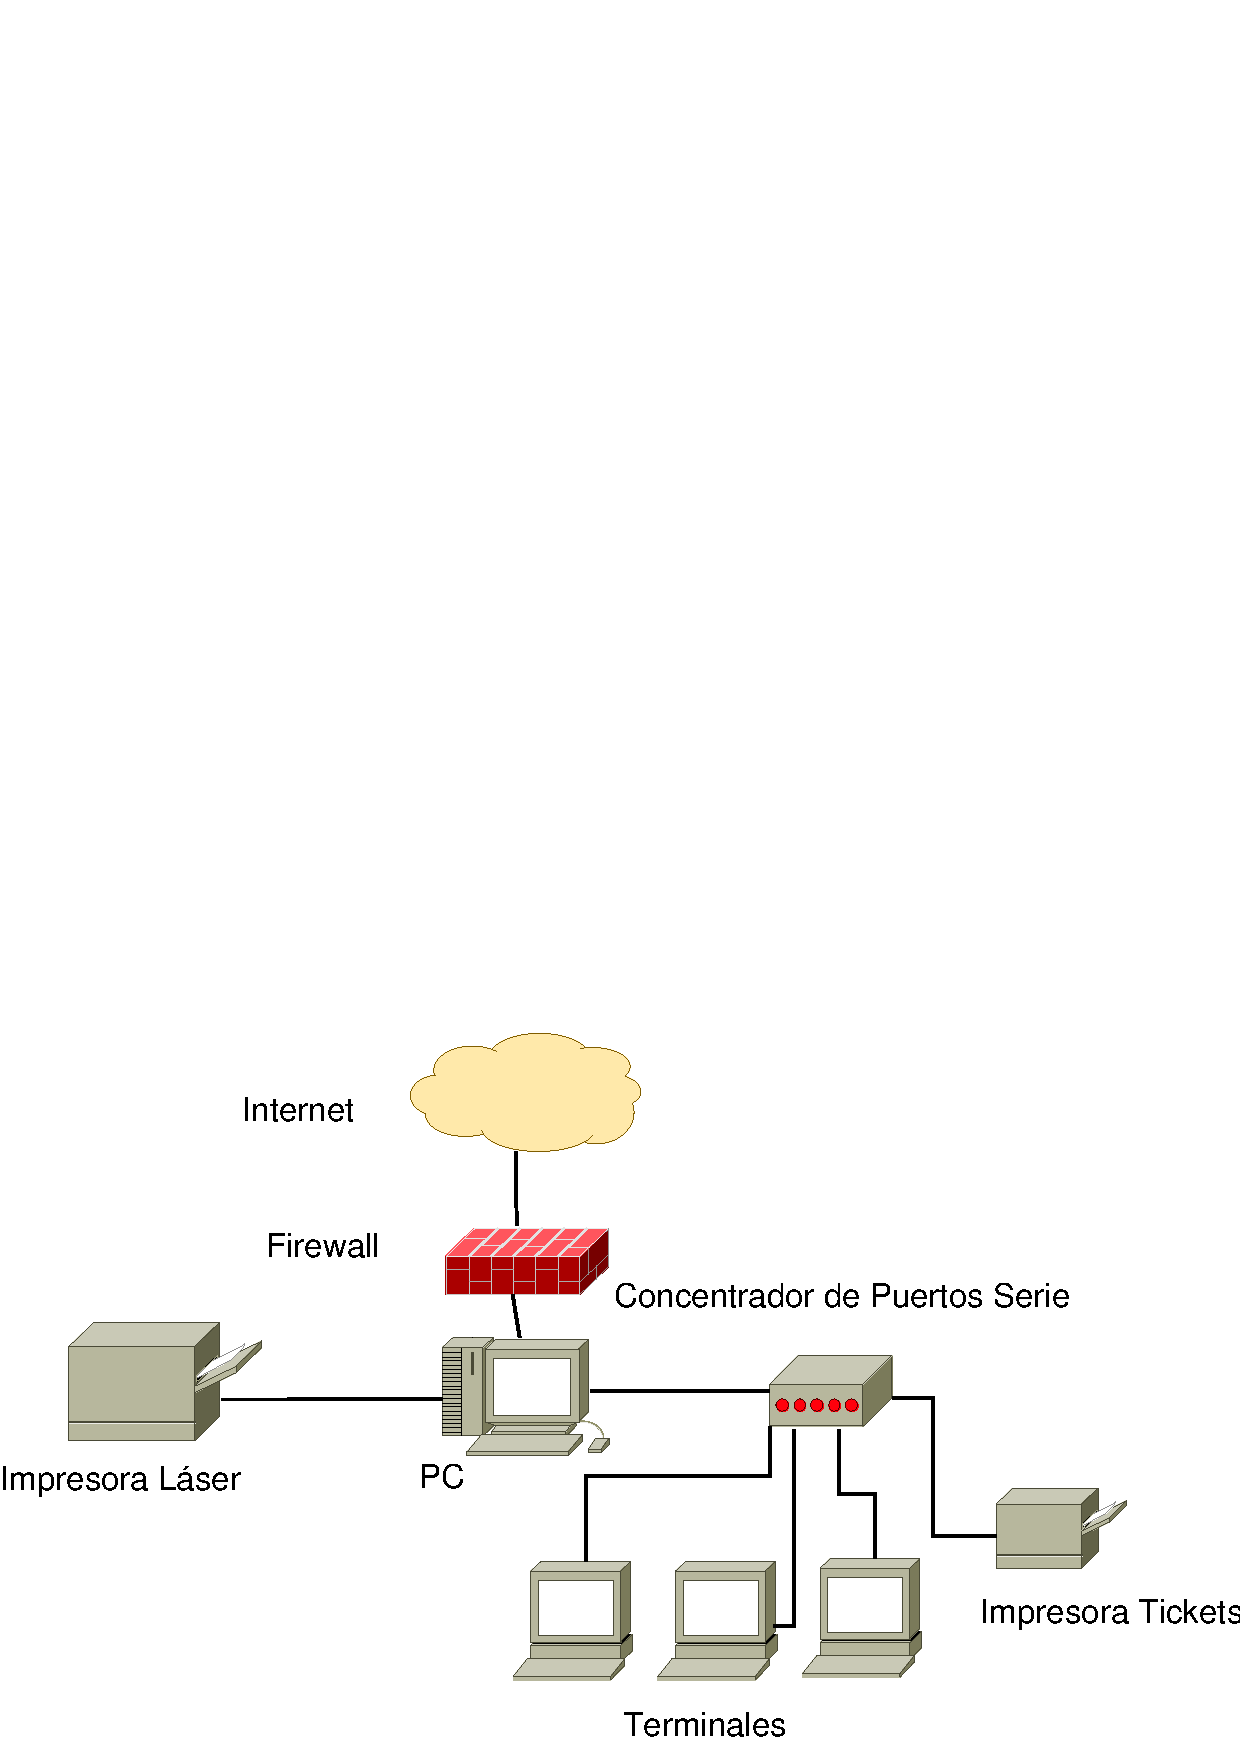
\includegraphics[scale=0.7]{diagrama_ph_sus_1.png}
 \end{center}
 \caption{Sistema en restaurantes PH}
 \label{fig:sist_rest_ph}
\end{figure}

El sistema se compone de una computadora en la cual se ejecuta el sistema punto de venta, se generan reportes propios del punto de venta, el gerente del restaurante consulta el correo electrónico, consulta reportes web propios del restaurante y de la intranet y realiza actividades propias de la operación (como cierres de inventarios, altas/bajas de empleados, etc.). Posee una impresora láser para imprimir documentos, reportes, etc.

La computadora tiene una conexión a internet protegida por un firewall y comunicación a la VPN\footnote{Virtual Private Network, red privada virtual} de la empresa.

Debido a la gran cantidad de equipo que se le puede conectar a la computadora, entre terminales, cajas registradoras e impresoras de tickets, principalmente, se hace uso de un concentrador de puertos seriales, a los cuales se conectan todos los dispositivos. Estos concentradores pueden ser de 6 o 12 puertos y pueden ser conectados más de uno, en caso necesario. La impresora es de matriz y se manda la impresión de los tickets una vez terminada de capturar la orden.

Las terminales, en caso de PH, sirven para tener el punto de venta, que se ejecuta en la computadora, en cada una de ellas, y así poder tomar varias ordenes al mismo tiempo.


La siguiente figura muestra el sistema en KFC a grandes rasgos:

\begin{figure}[htb]
 \begin{center}
  \includegraphics[scale=0.7]{diagrama_kfc_sus_1.png}
 \end{center}
 \caption{Sistema en restaurantes KFC}
 \label{fig:sist_rest_kfc}
\end{figure}

A diferencia del sistema en PH, se cuentan con cajas registradoras en lugar de terminales. Estas cajas registradoras son de la marca Panasonic, y se tienen dos modelos: touchscreen (Panasonic 790, que cuenta con sistema operativo Windows XP Embedded) para restaurantes con un gran número de transacciones y de teclado (Panasonic 5500, usando su propio firmware) para las demás. Se cuenta con un programa desarrollado en la empresa que convierte la salida de las cajas registradoras en registros de venta que son ingresados al punto de venta. Cada caja resgistradora cuenta con su propia impresora de tickets. Dentro del grupo de cajas registradoras se debe tener una especial llamada \textit{master}, la cual es la encargada de trasmitir programación a las secundarias, así como también de recibir información de venta de las demás cajas para ser impresas en el impresor de auditoría. A partir de un desarrollo realizado por mi, esta auditoría se dejó de imprimir y ahora es almacenada de manera electrónica.

\begin{figure}[htb]
 \begin{center}
  \includegraphics[scale=0.7]{panasonic_790.png}
 \end{center}
 \caption{Caja Panasonic 790}
 \label{fig:pana_790}
\end{figure}

\begin{figure}[htb]
 \begin{center}
  \includegraphics[scale=0.7]{panasonic_5500.png}
 \end{center}
 \caption{Caja Panasonic 5500}
 \label{fig:pana_5500}
\end{figure}


\section{Algunos Proyectos desarrollados}
\label{chap:desarrollo}

A continuación se presentan algunas actividades desarrolladas en la empresa.

\subsection{Auditoría Electrónica}
\label{sec:auditoria}

La operación del negocio debe ser vigilada por algún medio, en el cual se plasme un historial de ventas de cada caja registradora en KFC. Es por esto que se cuenta con un impresor de tickets llamado de auditoría, el cual imprime el resumen de venta de cada ticket de cada caja.

Una de las necesidades de negocio más importantes es la de reducción en el costo de venta. Por lo que se tomó la decisión de eliminar este impresor y almacenar la auditoría de manera electrónica. Con esto se ahorra los impresores de tickets, los gastos en mantenimiento de éstos y los rollos de papel en los más de 230 restaurantes KFC.

Ambos modelos de cajas cuentan con puertos seriales para conectar impresores, además de poseer con un puerto Ethernet RJ-45. Cada caja registradora cuenta con una dirección IP privada para la comunicación con la caja \textit{master}, la cual se encarga, a través de este medio, de transmitirles programación y de recibir los tickets de las demás cajas, para formar la auditoría. 

Por lo que se puede observar de esta descripción, es que hay dos maneras posibles de capturar la auditoría de la caja master: por el puerto serial que manda los datos al impresor, o mediante la captura de los paquetes de red que le llegan a la caja master provenientes de las demás cajas. Se optó por usar la salida del puerto seria hacia al impresor, ya que al mandar a imprimir se manda el ticket integro junto con los caracteres de control para la impresora. De la otra manera, se hubiese tenido que estudiar el protocolo de envío de información de las cajas a la caja master; lo que se sabe de manera certera, es que la comunicación es tipo UDP\footnote{User Datagram Protocol}.

Al estar configurada la caja master para manejar la auditoría, se debe especificar el puerto serie por el que se mandará a imprimir, en caso de no tener conectado un impresor, la caja marcará un error en su pantalla. Eso significa que la caja se encuentra continuamente solicitando un status a la impresora.

El concentrador de puertos seriales es el modelo AccelePort  Xem de la marca Digi, el cual posee 8 puertos tipo RJ-45, con posibilidad de aumentar el número de módulos para poder soportar más dispositivos.

\begin{figure}[htb]
 \begin{center}
  \includegraphics[scale=0.5]{acceleport_xem_lg.png}
 \end{center}
 \caption{AccelePort Xem de Digi con su tarjeta}
 \label{fig:digi}
\end{figure}

La configuración que indica el fabricante Digi para realizar un cable para impresora RJ-45 a DB-9 es el siguiente:


\begin{center}
 \resizebox{15cm}{!}{
  \begin{tabular}{|c|c|c|c|c|}
   \hline
   Pin RJ-45 & Señal & Dirección & Señal & Pin DB-9 \\
   \hline
   3 & GND (Tierra) & \textless\textendash\textgreater & GND (Tierra) & Carcaza \\
   \hline
   4 & TxD (Transmit Data) & \textendash\textgreater & RxD (Receive Data) & 2 \\
   \hline
   5 & RxD (Receive Data) & \textless\textendash & TxD (Transmit Data) & 3 \\
   \hline
   6 & SG (Signal Ground) & \textless\textendash\textgreater & SG (Signal Ground) & 5 \\
   \hline
   7 & CTS (Clear to Send) & \textless\textendash & DTR (Data Terminal Ready) & 4 \\
   \hline
   1 & DCD (Data Carrier Detect) & \textless\textendash & RTS (Request to Send) & 7 \\
   \hline
   2 & RTS (Request to Send) & \textendash\textgreater & CTS (Clear to Send) & 8 \\
   \hline
   8 & DTR (Data Terminal Ready) & \textendash\textgreater & DSR (Data Set Ready) & 6 \\
   \hline
  \end{tabular}
 }
\end{center}

Para poder saber qué datos manda la caja hice uso de un cable con el que se pueda leer la comunicación de la caja registradora (DB-9) al impresor de auditoría (DB-25). Por lo que abrí el cable e inserté las líneas descritas en la configuración anterior para un RJ-45, de esta manera se cuenta con un cable capaz de leer los datos mandados por la caja registradora. Para la lectura de estos datos utilice el software \textit{minicom}. Este es un programa de software libre utilizado para monitorear el puerto serie, análogo al \textit{Hyperterminal} de Windows. Los resultados indicaron que la caja manda el ticket con únicamente la información necesaria como número de productos, el producto, el costo del producto, el subtotal, el total, fecha, hora, número de ticket y el cajero que lo tomó. Además de estos datos, se cuentan con caracteres de control especiales para el impresor.

Otra característica que observé fue que la caja constantemente se comunica con el impresor para saber si está conectado y este último le manda una respuesta. Por lo que el programa desarrollado en C tendría que: limpiar los caracteres de control, y emular la comunicación que establece la caja registradora par evitar que marque error.

El cable original que va de la caja (DB-9) al impresor (DB-25) tiene la siguiente configuración:

\begin{center}
  \begin{tabular}{|c|c|c|c|}
   \hline
   Pin DB-9 & Señal DB-9 & Pin DB-25 & Señal DB-25 \\
   \hline
   1 &  DCD & 4 y 5 & RTS y CTS \\
   \hline
   2 & RxD & 2 & TxD \\
   \hline
   3 & TxD & 3 & RxD \\
   \hline
   4 & DTR & 6 y 22 & DSR y Ring indicator \\
   \hline
   5 & SG & 7 & SG \\
   \hline
   6 y 9 & Ring indicator y DSR & 20 & DTR \\
   \hline
   7 y 8 & CTS y RTS & 8 & DCT \\
   \hline
  \end{tabular}
\end{center}

De acuerdo a la configuración anterior y la indicada por el fabricante para el cable DB-9 a RJ-45, realicé la siguiente configuración de cable:

\begin{center}
 \begin{tabular}{|c|c|}
  \hline
  RJ-45 & DB-9 \\
  \hline
  1 & 7 y 8 \\
  \hline
  2 & 4 \\
  \hline
  3 & carcaza \\
  \hline
  4 & 2 \\
  \hline
  5 & 3 \\
  \hline
  6 & 5 \\
  \hline
  7 & 4 \\
  \hline
  8 & 6 \\
  \hline
 \end{tabular}
\end{center}

Desarrollé en lenguaje C el programa que lee los datos de la caja y además emula la respuesta del impresor a la caja. El programa \textit{portAudit} recibe como argumento el puerto serie del concentrador en el cual está conectado el cable. El programa \textit{portAudit} recibe como variable de ambiente el tipo de caja: \texttt{PORT\_TIPO\_CAJA=790} y \texttt{export PORT\_TIPO\_CAJA=5500} ya que los caracteres de control son distintos para cada caja registradora. Creé un script encargado de establecer estas variables, la configuración del puerto serial (velocidad, paridad, etc.) y la ejecución del binario.

El programa detecta la caja que originó el ticket, y de acuerdo a esta información la almacena en un archivo de texto para cada caja, además de un archivo que concentra la información de todas las cajas.

De acuerdo a la versión del sistema operativo en restaurantes, añadí una entrada en el archivo \texttt{/etc/inittab} para poder controlar de manera automática el inicio del servicio de almacenamiento de auditoría de manera automática de acuerdo al nivel de ejecución del sistema. 

A continuación se muestran dos tickets de ejemplo de auditoría:

\begin{Verbatim}[fontsize=\small]
    #335                 LLEV  
 4 MIXTA   
 1 PQ8BI SE                125.00  
   1 PAPFADO                35.00  
   1 NINGUNO                  .01  
           VTPR            160.00  
           TOTL       160.00  
           EFVO            200.00  
           CAMB             40.00  
NACHO  
  8377 10:51 #12 MAR.01'11  REG0003  
 


    #336                 COME  
 1 MBBIG C                  72.00  
   1 +PUR/RE                 7.00  
   1 NINGUNO                  .01  
 1 MANZANA   
           TOTL         79.00  
           EFVO            100.00  
           CAMB             21.00  
NACHO  
  8378 11:20 #12 MAR.01'11  REG0003  
\end{Verbatim}

Los tickets número 335 y 336 indican que provienen de la caja 3. El \#335 es un pedido para llevar y el \#336 es para comer en el restaurante. Se muestran las cantidades de los productos, su precio, el total, el efectivo con que se pagó y el cambio, el número de ticket único, así como la fecha y hora. El ticket \#335 que se manda a imprimir para dárselo al cliente se muestra a continuación:

\begin{Verbatim}[fontsize=\small]
 PREMIUM RESTAURANT BRANDS SDE RL DE CV  
     PASEO DE TAMARINDOS 400 PISO1       
   BOSQUES DE LAS LOMAS, CUAJIMALPA      
          MEXICO, D.F. 05120             
           RFC PRB100802H20              
--------------------------------------   
 #335       LLEV  
 4 MIXTA   
 1 PQ8BI SE                125.00  
 1 PAPFADO                  35.00  
 1 NINGUNO                   0.00  
          -------------------------  
           TOTAL A PAGAR     160.00  
Ciento Sesenta Pesos 00/100 M.N.  
           EFVO            200.00  
           CAMB             40.00  
                                         
      Sucursal KFC Div. del Norte        
      AV. DIVISION DEL NORTE 2855        
      PARQUE SAN ANDRES C.P.04040        
        MEXICO,DISTRITO FEDERAL          
NACHO  
  8377 10:51 #12 MAR.01'11  REG0003  
          No. ticket unico: 6     
    (solo se factura el mismo dia)       
         Gracias por su compra           
\end{Verbatim}

Para la verificación del correcto funcionamiento del \texttt{portAudit} creé un script que valida que todas las cajas estén registrando auditoría, y que no falte ningún ticket. Esto se realiza verificando primero, la existencia de la auditoría de las cajas en donde ya haya habido venta, después se busca el número de ticket en los archivos generados por la interfase que convierte la información de la caja registradora al punto de venta, y se revisa que en la auditoría correspondiente a la caja se encuentre. En caso de que no esté en ejecución el \texttt{portAudit}, que no se estén generando los archivos de auditoría o falten tickets de auditoría se genera un correo electrónico de manera automática para avisar de la situación correspondiente. Este script se ejecuta mediante CRON cada veinte minutos.

Ejemplo de correo electrónico cuando falta el archivo de auditoría de alguna caja:

\begin{Verbatim}[fontsize=\tiny]
Received: from xxxxxxxx.xxx.com.mx (192.168.101.xxx) by xxxxxxxx.xxx.com
 (xxx.xxx.xxx.xxx) with Microsoft SMTP Server id 14.0.639.21; Mon, 13 Jun 2011
 15:00:31 -0500
Received: from xxxx.xxx.com.mx (unknown [xx.xxx.xx.xxx])	by
 linuxeon.prb.com.mx (Postfix) with ESMTP id 07CCC2531;	Mon, 13 Jun 2011
 15:00:29 -0500 (CDT)
From: <mx0628r@xxx.com.mx>
To: <sergio.cuellar@xxx.com.mx>, <anibal.avelar@xxx.com.mx>,
	<jesus.noriega@xxx.com.mx>, <juanjose.martinez@xxx.com.mx>,
	<yaneth.yanez@xxx.com.mx>, <hugo.jacobo@xxx.com.mx>
Message-ID: <10776760.0.1307977209538.JavaMail.root@S062801>
Subject: Port de Auditoria CC 0628 13-06-2011-15:00: FALTA ARCHIVO DE ALGUNA
 CAJA
Content-Type: text/plain; charset="ISO-8859-1"
Content-Transfer-Encoding: 7bit
Date: Mon, 13 Jun 2011 15:00:29 -0500
Return-Path: mx0628r@xxx.com.mx
X-MS-Exchange-Organization-AuthSource: mexxch02.xxx.com
X-MS-Exchange-Organization-AuthAs: Anonymous
MIME-Version: 1.0

Falta(n) archivo(s) de auditoria de caja(s):
04


* Revisar banderas de cajas
* Revisar conexion de cables
* Revisar concentrador
\end{Verbatim}

El gerente del restaurante puede revisar los tickets de auditoría y del punto de venta mediante un reporte tipo web, en donde le indica la fecha que requiere consultar y como opción tiene la de ingresar el número de ticket a buscar, en caso de que no ingrese este dato, se despliegan todos los tickets del día. Esto se logra gracias a que los tickets de auditoría son almacenados en un directorio específico. El reporte consulta el archivo de acuerdo a la fecha seleccionada. 

\begin{figure}[htb]
 \begin{center}
  \includegraphics[scale=0.5]{ticket_audit_ereports.png}
 \end{center}
 \caption{Resultado de una consulta al reporte web de Ticket de Auditoría}
 \label{fig:rep_audit_ereports}
\end{figure}

Con esta solución se ha tenido un gran ahorro económico derivado de dejar de consumir papel, cintas de tinta, impresores y su mantenimiento. Igualmente se tiene un impacto benéfico a la ecología, ya que se deja de utilizar una cantidad importante de papel, teniendo una auditoría \textit{paperless}.

\subsection{Reporte de Estimado de Usos Ideales en KFC}
\label{sec:usos_ideales_kfc}

En KFC (y Pizza Hut) se necesita saber con anticipación el número de transacciones que se tendrán para cada día, de esta manera se puede saber, mediante un pronóstico, el número de hamburguesas que se deben preparar, el número de piezas de pollo que se deben marinar para posteriormente cocinarlas, el número de purés que se deben tener listos, etc. De esta manera la operación del restaurante está preparada para el nivel de transacciones que se tengan durante el día. Sabiendo esto, el gerente sabe el nivel de inventario que debe tener para satisfacer las transacciones, el número de piezas de pollo que debe descongelar, el número de asociados (empleados) que debe tener a cierta hora del día para poder preparar los productos, etc. 

El uso ideal es la cantidad de producto que el restaurante tuvo que haber usado, de acuerdo a su número de transacciones, y a la cantidad de producto establecida por la receta, sin incluir la merma. La merma son los productos, ingredientes o artículos que deben ser descartados debido a: deterioro, han expirado o se produjeron en exceso. La diferencia entre el uso ideal y el uso actual se le conoce como varianza, y puede ser expresada en cantidad de productos o en su valor monetario. Si la varianza es negativa significa que un producto o ingrediente fue utilizado más que la cantidad ideal; si es positiva, un producto o ingrediente fue utilizado menos que lo que dice el ideal.

El uso ideal se conoce una vez que han cerrado las ventas para el día y se generan los reportes del punto de venta. Para el gerente de restaurante es importante saber cuántos vasos, tapas, panes, kilos de papa debe tener listos para la operación de un día específico. Para esto debe conocer el pronóstico en el número de transacciones que tendrá para un día específico. No es lo mismo un domingo que un martes, ni un 16 de diciembre, que un 24 de diciembre. Una vez conocido el número de transacciones pronosticadas, el gerente, debe investigar cuál día tuvo ese número de transacciones, pero ahora reales. Una vez hecho esto debe consultar un reporte de esa fecha generado por el punto de venta donde se encuentran los usos ideales y obtener de el reporte el uso ideal de los productos que necesite.

Esto ocasiona que el gerente ocupe mucho tiempo en la búsqueda de estos usos ideales, por lo que desarrollé un reporte que automatice esta actividad.

Para facilitar la elaboración de este reporte, creé una tabla en la base de datos de PostgreSQL que almacene los usos ideales por fecha y por identificador de producto. Estos datos se obtiene de un comando que ya existe en el sistema y mediante un script en Perl se parsean los resultados y se ingresan a la base de datos. Esta carga se realiza de manera diaria, una vez que se han generado los usos ideales del día anterior. 

Esta es la descripción de la tabla de PostgreSQL encargada de almacenar los usos ideales:

\begin{Verbatim}[fontsize=\tiny]
    Table "public.op_inv_ideal_use"
  Column   |     Type      | Modifiers 
-----------+---------------+-----------
 turn_date | date          | not null
 turn_id   | smallint      | not null
 inv_id    | character(6)  | not null
 ideal_use | numeric(12,2) | 
 unit_cost | numeric(12,2) | 
 misc      | boolean       | 
Indexes:
    "op_invc_ideal_use_pkey" PRIMARY KEY, btree (turn_date, turn_id, inv_id)
Foreign-key constraints:
    "fk1" FOREIGN KEY (inv_id) REFERENCES op_grl_cat_inventory(inv_id) ON UPDATE RESTRICT ON DELETE RESTRICT
\end{Verbatim}

La llave foránea \texttt{inv\_id} pertenece a la tabla \texttt{op\_grl\_cat\_inventory}, la cual contiene, entre otros datos, el nombre del producto y la unidad de medida.

El los restaurantes existe una aplicación llamada \textit{e-Reports}\pageref{sec:ereports}, la cual está desarrollada en JSP\footnote{Java Server Pages}. En está aplicación se añaden los reportes requeridos clasificándolos de acuerdo a su finalidad. El reporte de ``Usos Ideales'' se  encuentra en el menú de \textit{Mano de Obra \textendash\textgreater Planeación \textendash\textgreater Usos Ideales Diarios}.

Creé archivos de configuración de productos clasificados de acuerdo a la línea de producción donde son utilizados. Los archivos son:

\begin{itemize}
 \item Biscuits.conf
 \item Ensalada.conf
 \item Marinado.conf
 \item Pure.conf
 \item Sandwich.conf
 \item Trasempaque.conf
 \item Congelados.conf  
 \item Home\_Delivery.conf
 \item Pure\_Ensalada.conf  
 \item Servicio.conf
\end{itemize}

En ellos se encuentra el número de inventario del producto a deplegar en el reporte. A continuación se muestra una parte del archivo de \texttt{Servicio.conf}:

\begin{Verbatim}[fontsize=\small]
#####################
###   Servicio    ###
#####################
# Caja regular
10519
# Tapa vaso 12 oz
10738
# Caja Economica
10517
# Servilletas
10570
# Tapa 32 oz
10830
# Bucket
10946
# caja chicky
10593
# Char porta vaso
10613
# Catsup sobre
10559
\end{Verbatim}

Teniendo estos archivos de configuración resulta muy fácil añadir o quitar productos de acuerdo a las necesidades de la operación.

El reporte obtiene de la tabla \texttt{op\_gt\_real\_sist\_mng} el pronóstico de número de transacciones y las transacciones reales más cercanas a la fecha seleccionada.

A continuación se muestra una pantalla de resultados del reporte:

\begin{figure}[htb]
 \begin{center}
  \includegraphics[scale=0.5]{ideal_use_2.png}
 \end{center}
 \caption{Usos Ideales Diarios en KFC}
 \label{fig:usos_ideales_kfc}
\end{figure}

\subsection{Cierre de Lote de Tarjeta de Crédito}
\label{sec:cierre_lote}

El uso de tarjetas de crédito y débito es indispensable para cualquier negocio ya que al no aceptarlas se pueden perder valiosas transacciones. Las tarjetas, hoy en día, no sólo son un método o forma de pago, sino que da seguridad a quienes la aportan, tanto seguridad al no portar efectivo como seguridad de poder pagar a largo plazo en caso de que no cuenten con el dinero, además de poder tener diferentes beneficios con sus puntos que otorga el banco al realizar compras, como viajes, artículos entre otros.

Actualmente la compañía ya cuenta con el servicio de cobro de tarjetas en la marca PH y se encuentra en un mercado prueba para la marca KFC, ambos obtuvieron excelentes resultados, tanto en transacciones como en un aumento en el ticket promedio por lo que se ha tomado la
decisión de realizar el lanzamiento nacional por fases hasta cubrir el 100\% de los restaurantes.

Existe una actividad muy importante que se debe realizar siempre al final del día, una vez que han concluido las ventas, el cierre de lote en las terminales bancarias. Con el cierre de lote se asegura que el banco depositará el dinero correspondiente a las ventas pagadas mediante tarjeta de crédito/débito, al siguiente día hábil. La importancia de esta actividad radica en las conciliaciones bancarias que se deben realizar de manera diaria, un retraso en el pago de este dinero ocasiona que no se puedan realizar a tiempo estas conciliaciones.

Por esta razón, la necesidad del negocio requiere de una aplicación en la cual los asociados ingresen el monto total cobrado de cada terminal bancaria, forzándolos ha haber realizado el cierre de lote en cada dispositivo. La aplicación fue desarrollada para \textit{e-Reports}.

Los únicos asociados autorizados para realizar el cierre de lote, son aquellos que poseen un nivel de seguridad 1 en el sistema de punto de venta. Creé una tabla en la base de datos de PostgreSQL (\texttt{ss\_cat\_terminals\_ccard}) que contiene información relacionada al número de terminales bancarias con el que cuenta el restaurante. De esta manera, únicamente se despliegan el número de terminales bancarias con las que cuente el restaurante.

Los datos que deben ser ingresados por cada terminal bancaria son:

\begin{itemize}
 \item Monto que indica el cierre de lote de la terminal. En caso de no haber cobrado con una terminal se debe ingresar \texttt{0.0}.
 \item Fecha en que se realiza el cierre de lote.
 \item Hora en que se realiza el cierre de lote.
 \item Número de transacciones que reporta la terminal.
 \item El campo de ``Cierre Fallido`` se utiliza en caso de que haya existido un error en la terminal bancaria, por ejemplo, por problemas de comunicación.
\end{itemize}

Una vez ingresados estos datos, se debe presionar el botón de \texttt{Obtener montos totales}, con esta acción, se obtiene la cantidad total de dinero registrado en las terminales bancarias y el total de ventas cobradas con tarjeta de crédito/débito que se tienen registrados en el sistema punto de venta. Estos totales, deben coincidir, en caso de no hacerlo, se muestra un mensaje indicando la diferencia y sugiriendo revisar los datos, y si es el caso, corregirlos. Después se debe presionar el botón de \texttt{Guardar y confirmar datos}, en esta parte es cuando se le solicita al asociado, elegir su nombre de usuario y teclear su contraseña. Una vez realizado esto de manera correcta se almacenarán los datos ingresados y en caso de haber exisitido diferencia entre los montos totales del sistema punto de venta y el de las terminales bancarias se manda un correo electrónico automático al restaurante, al gerente de zona y a las personas del área de Ingresos correspondientes.


\begin{figure}[htb]
 \begin{center}
  \includegraphics[scale=0.7]{cierre_lote_1.png}
 \end{center}
 \caption{Cierre de Lote de Tarjeta de Crédito en e-Reports}
 \label{fig:cierre_lote_1}
\end{figure}

Existe además, una alarma que funciona a manera de recordatorio, en caso de que no se haya realizado el cierre de lote a las 23:45 horas. La alarma, realizada en Perl y Xdialog, consiste en una ventana que aparece en la computadora del restaurante recordando ingresar los datos del cierre de lote, así como también la generación de \textit{beeps} en la misma computadora, y en caso de ser restaurante PH, en todas las terminales. Al desactivar la alarma, ésta solicitará por el usuario y contraseña de quien lo está realizando, esto con el fin de almacenar esta información en un archivo. En caso de que nadie la desactive, ésta automáticamente se apaga después de 15 minutos.

\begin{figure}[htb]
 \begin{center}
  \includegraphics[scale=0.7]{cierre_lote_4.png}
 \end{center}
 \caption{Ventanas de Xdialog de la alarma}
 \label{fig:cierre_lote_4}
\end{figure}

Cada cierre de lote realizado en \textit{e-Reports} es almacenado en un archivo, con lo cual se puede tener un registro de este reporte. A continuación se muestra un ejemplo de archivo almacenado:

\begin{Verbatim}[fontsize=\small]
222|1|11-05-14|11-05-14|20:52|4874.20|5190.2|5190.2|0.0|28|SENI|14-5-2011 21:16:13
222|2|11-05-14|11-05-14|21:10|316|5190.2|5190.2|0.0|1|SENI|14-5-2011 21:16:13
222|3|11-05-14|11-05-14|00:00|0|5190.2|5190.2|0.0|0|SENI|14-5-2011 21:16:13
222|4|11-05-14|11-05-14|00:00|0|5190.2|5190.2|0.0|0|SENI|14-5-2011 21:16:13
\end{Verbatim}

Los campos indican:

\begin{description}
 \item[Primer campo] es el número del restaurante.
 \item[Segundo campo] es el número de terminal bancaria.
 \item[Tercer campo] es la fecha en la que se capturó el cierre de lote.
 \item[Cuarto campo] es la fecha negocio, la cual es la fecha que tiene el sistema punto de venta. En algunos casos puede que no coincida la fecha actual con la fecha de negocio.
 \item[Quinto campo] es la hora que marca la terminal bancaria al momento de realizar el cierre de lote.
 \item[Sexto campo] es el monto cobrado en la terminal bancaria.
 \item[Séptimo campo] es el monto total cobrado de las terminales bancarias.
 \item[Octavo campo] es el monto total que reporta el sistema punto de venta que fue pagado con tarjeta de crédito/débito.
 \item[Noveno campo] es la diferencia entre el monto total que reporta el sistema punto de venta y monto total cobrado de las terminales bancarias.
 \item[Décimo campo] es el número de transacciones cobradas en la respectiva terminal bancaria.
 \item[Onceavo campo] es el nombre de usuario que realizó el cierre de lote.
 \item[Doceavo campo] es el timestamp del sistema al momento de realizar el cierre de lote.
\end{description}